\chapter{OSDOCR Editor - Implementação}
\label{cap_osdocr_editor_implementacao}


% proposito e ferramentas utilizadas

% funcionalidades disponiveis
%% abir diferentes resultados OCR para uma mesma imagem
%% mover blocos singularmente ou em grupo
%% ajustar dimensoes de blocos
%% OCR de bloco
%%% configuracoes de OCR
%% configuracoes de editor
%% dividir bloco manualmente
%% dividir bloco por espaços vazios
%% categorizar blocos manualmente
%% ordenar blocos
%% calcular ordem de blocos
%% gerar artigos automaticamente
%% gerir artigos
%%% adicionar e remover
%%% adicionar e remover blocos a artigos
%%% alterar ordem dos artigos
%% gerar output
%%% simples
%%% markdown
%%% OCR Tree
%% cache de operacoes
%%% retroceder e reconstruir operacoes





% \section{GUI Simples}
% \label{gui_simples}
% 
% De forma a facilitar a visualização dos resultados dos motores OCR, assim como das transformações realizadas nestes pelas diferentes técnicas aplicadas, foi implementado um GUI simples em Python utilizando a biblioteca PySimpleGUI. Isto tornou o processo de análise dos dados mais intuitiva e interativa, principalmente no processo de manipulação de blocos.
% 
% O formato da interface gráfica é relativamente simples, servindo principalmente o uso de debugging. Esta permite:
% 
% \begin{itemize}\setlength\itemsep{0.05cm}
%     \item Escolha de ficheiro de input - ficheiros imagem
%     \item Aplicação de reconhecimento na imagem - utilizando Tesseract
%     \item Visualizar blocos dos resultados
%     \item Visualizar texto de bloco
%     \item Aplicar funcionalidades e visualizar resultados
%     \begin{itemize}
%         \item Limpeza de blocos
%         \item Ordenação de caixas
%         \item Extração de artigos
%         \item Cálculo de template de jornal utilizando delimitadores
%     \end{itemize}
% \end{itemize}
% 
% Seguem-se alguns exemplos da interface:
% 
% \subsubsection{Interface gráfica}
% 
% \begin{figure}[H]
%     \centering
%     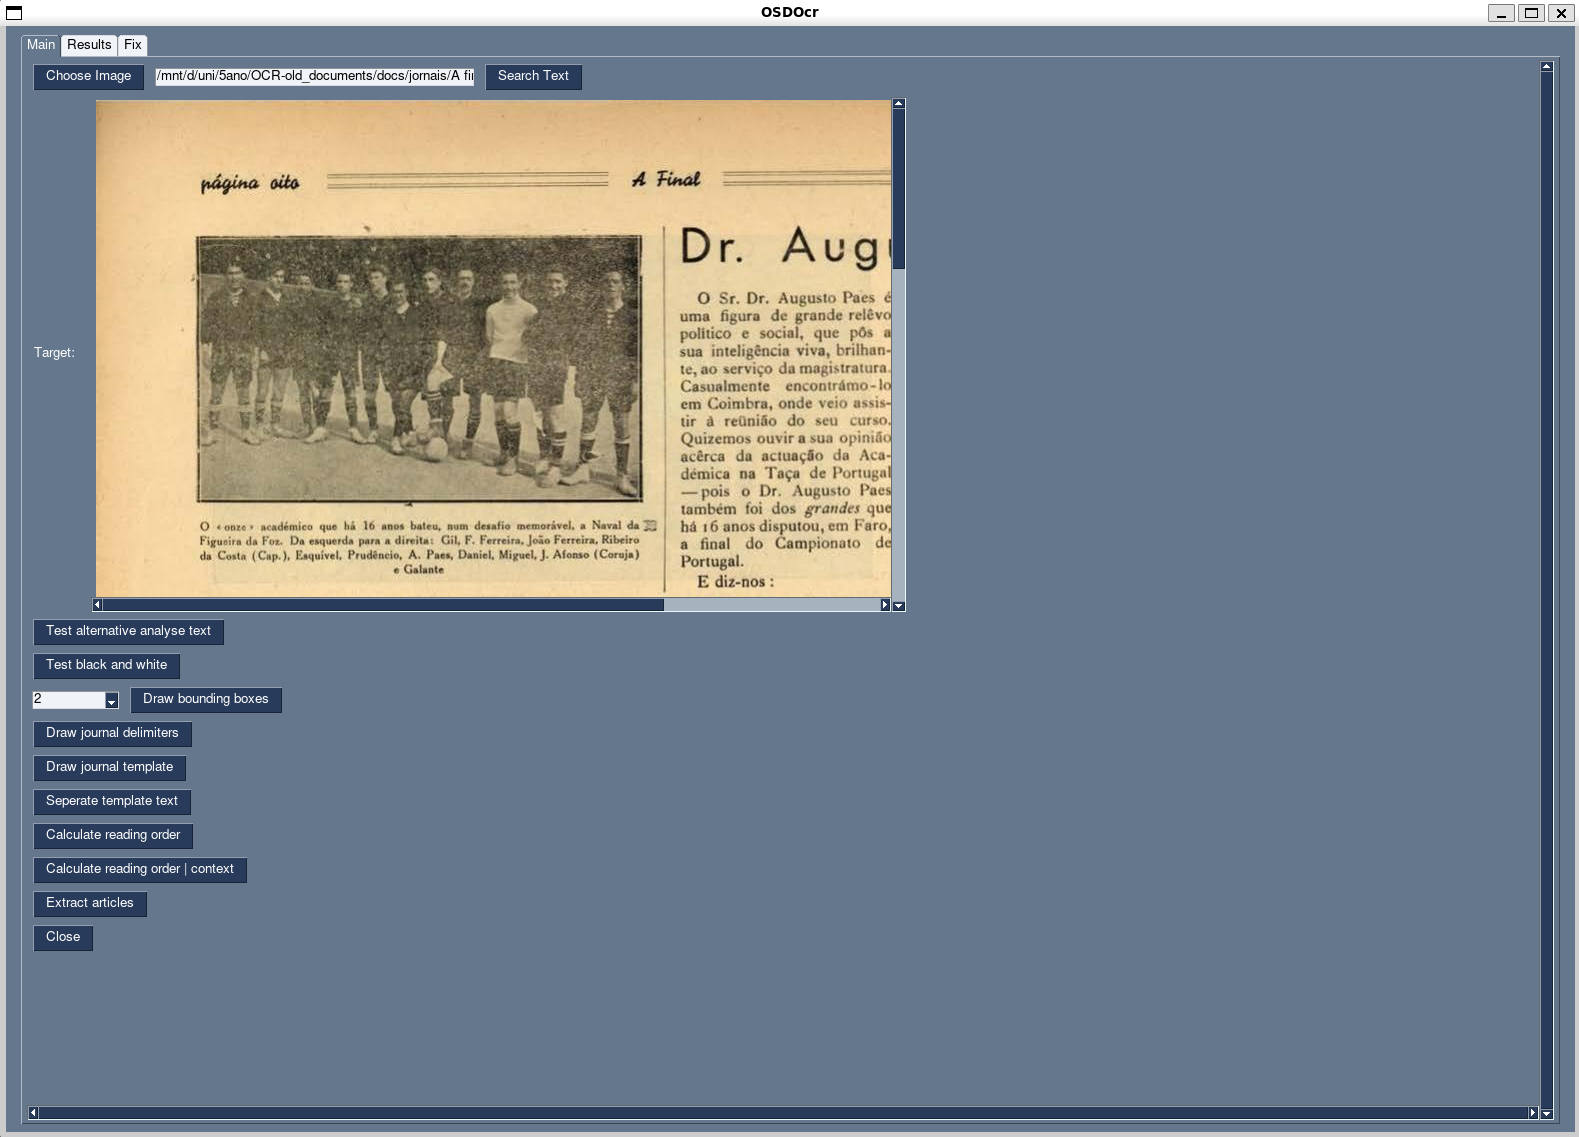
\includegraphics[width=1\textwidth]{images/implementacao/gui/gui_base.png}
%     \caption{Interface gráfica simples}
%     \label{fig:gui_base}
% \end{figure}
% 
% \subsubsection{Visualização de bounding boxes}
% 
% \begin{figure}[H]
%     \centering
%     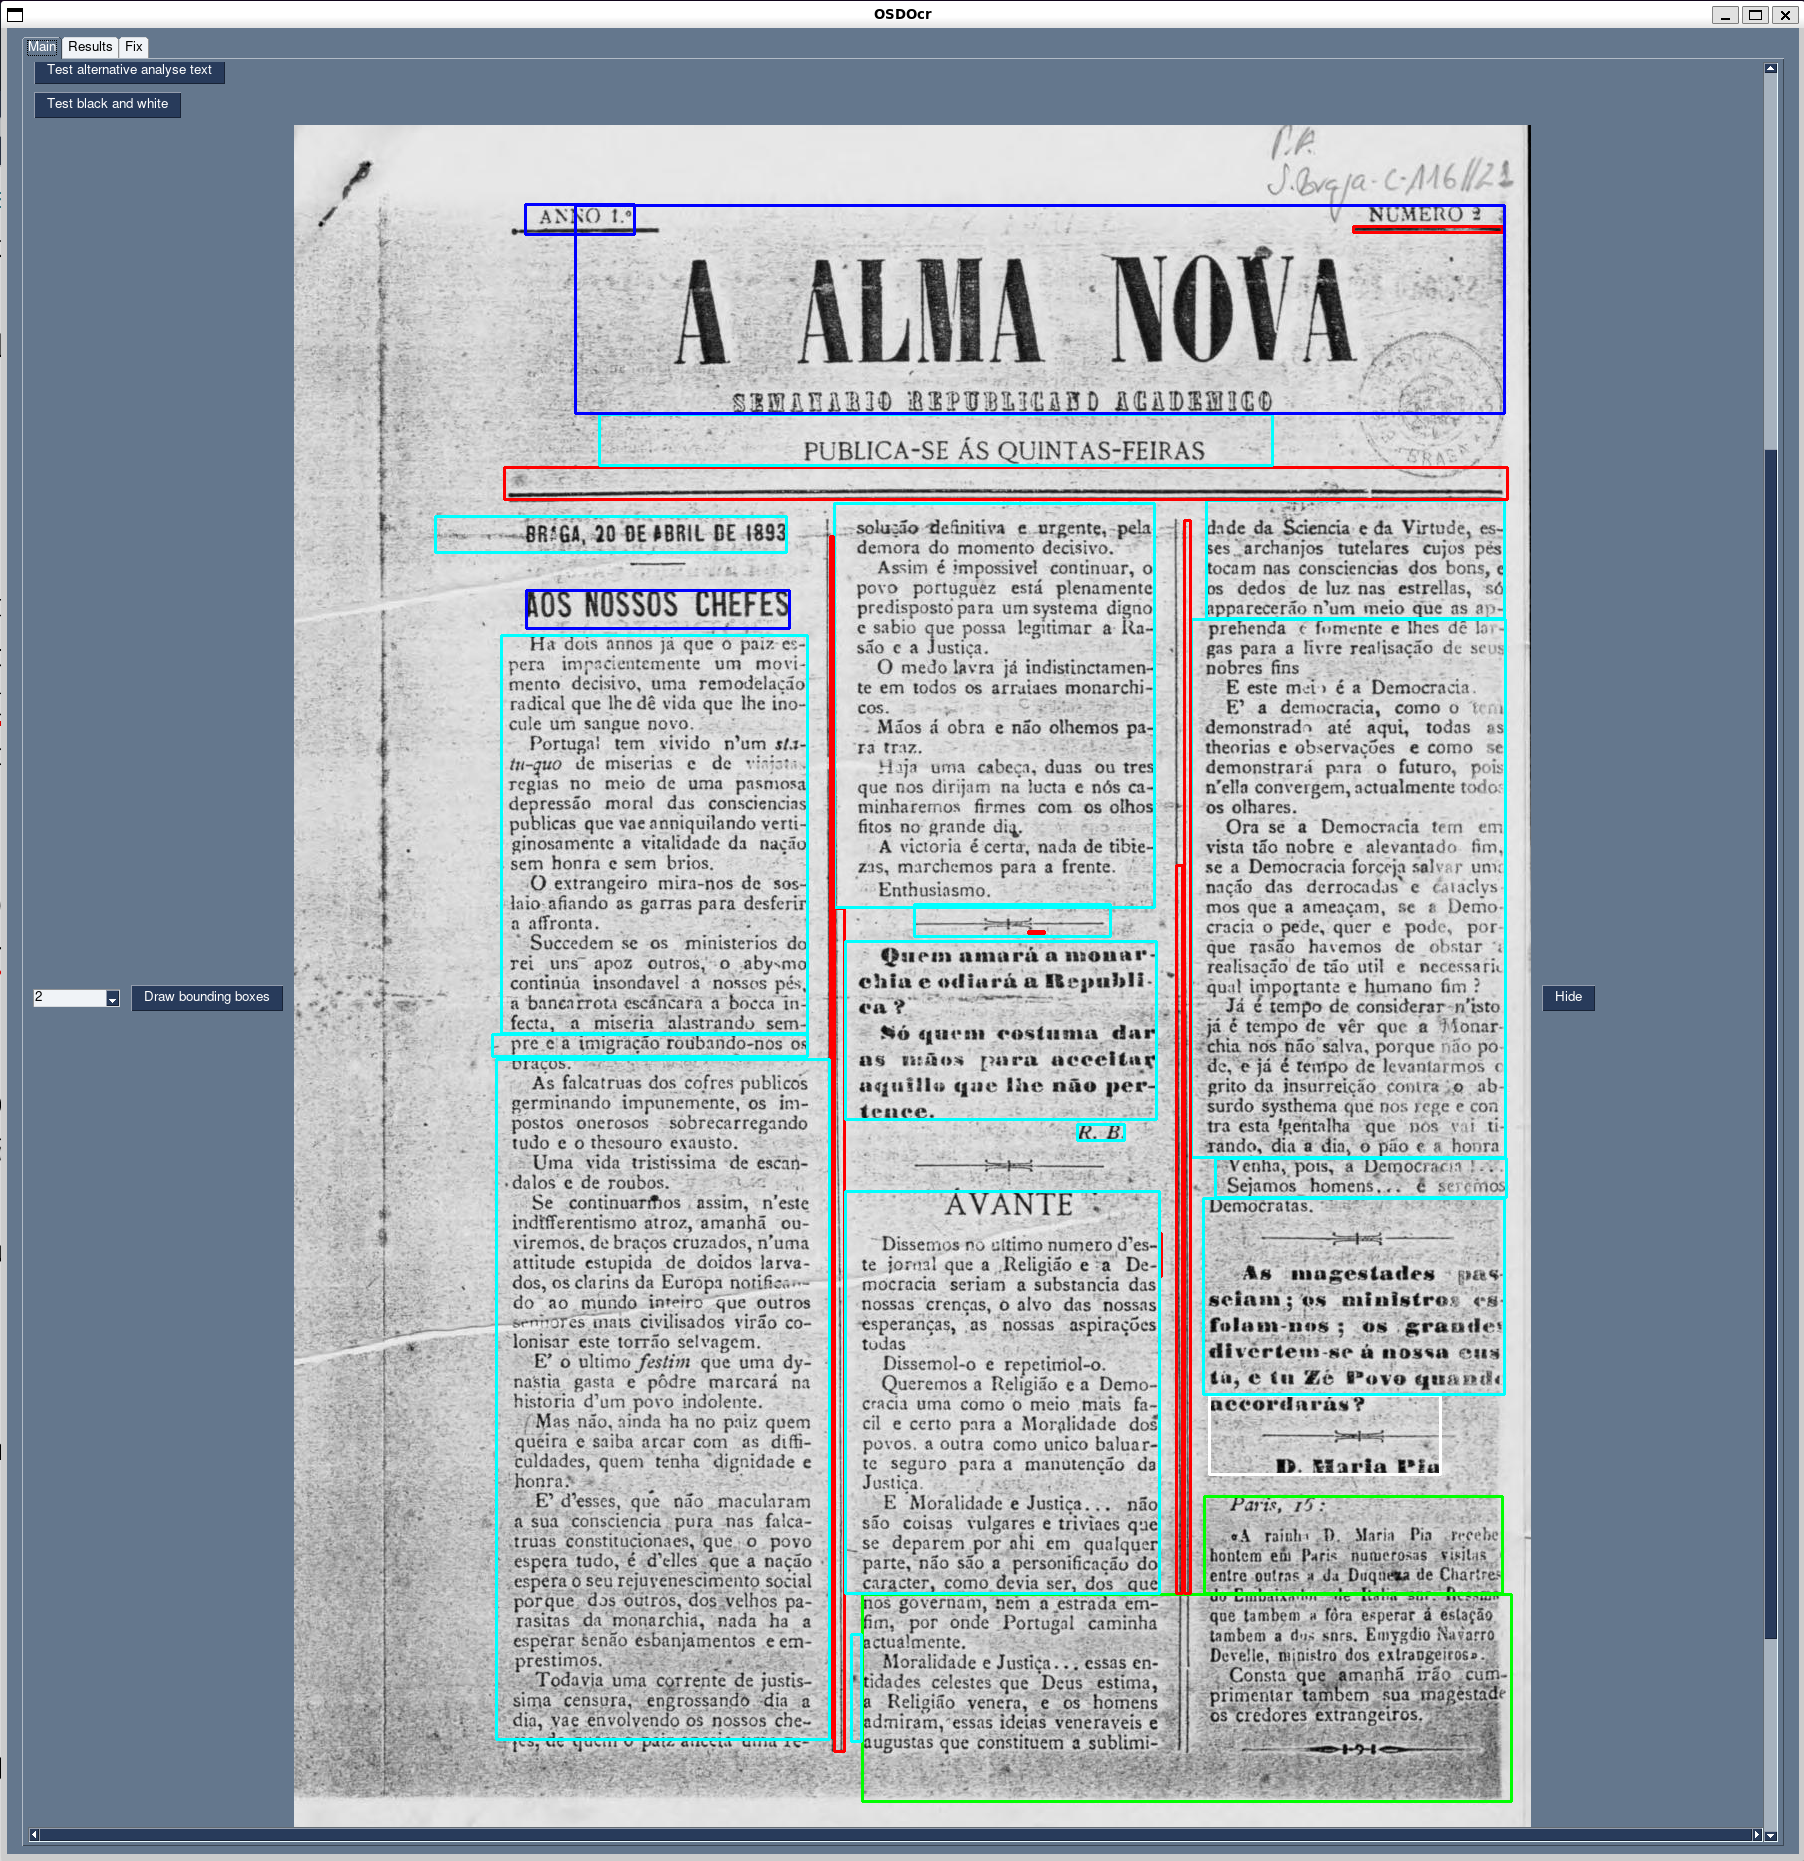
\includegraphics[width=1\textwidth]{images/implementacao/gui/gui_draw_bb.png}
%     \caption{Visualização dos blocos resultantes de OCR}
%     \label{fig:gui_draw_bb}
% \end{figure}
% 
% A visualização de blocos dispõe também de coloração diferente para os blocos de acordo com a sua categorização. Blocos título estão a azul escuro, texto a azul claro, delimitadores a vermelho, legendas a branco e o resto - imagens, outros - a verde.
% 
% \subsubsection{Cálculo de template de jornal}
% 
% \begin{figure}[H]
%     \centering
%     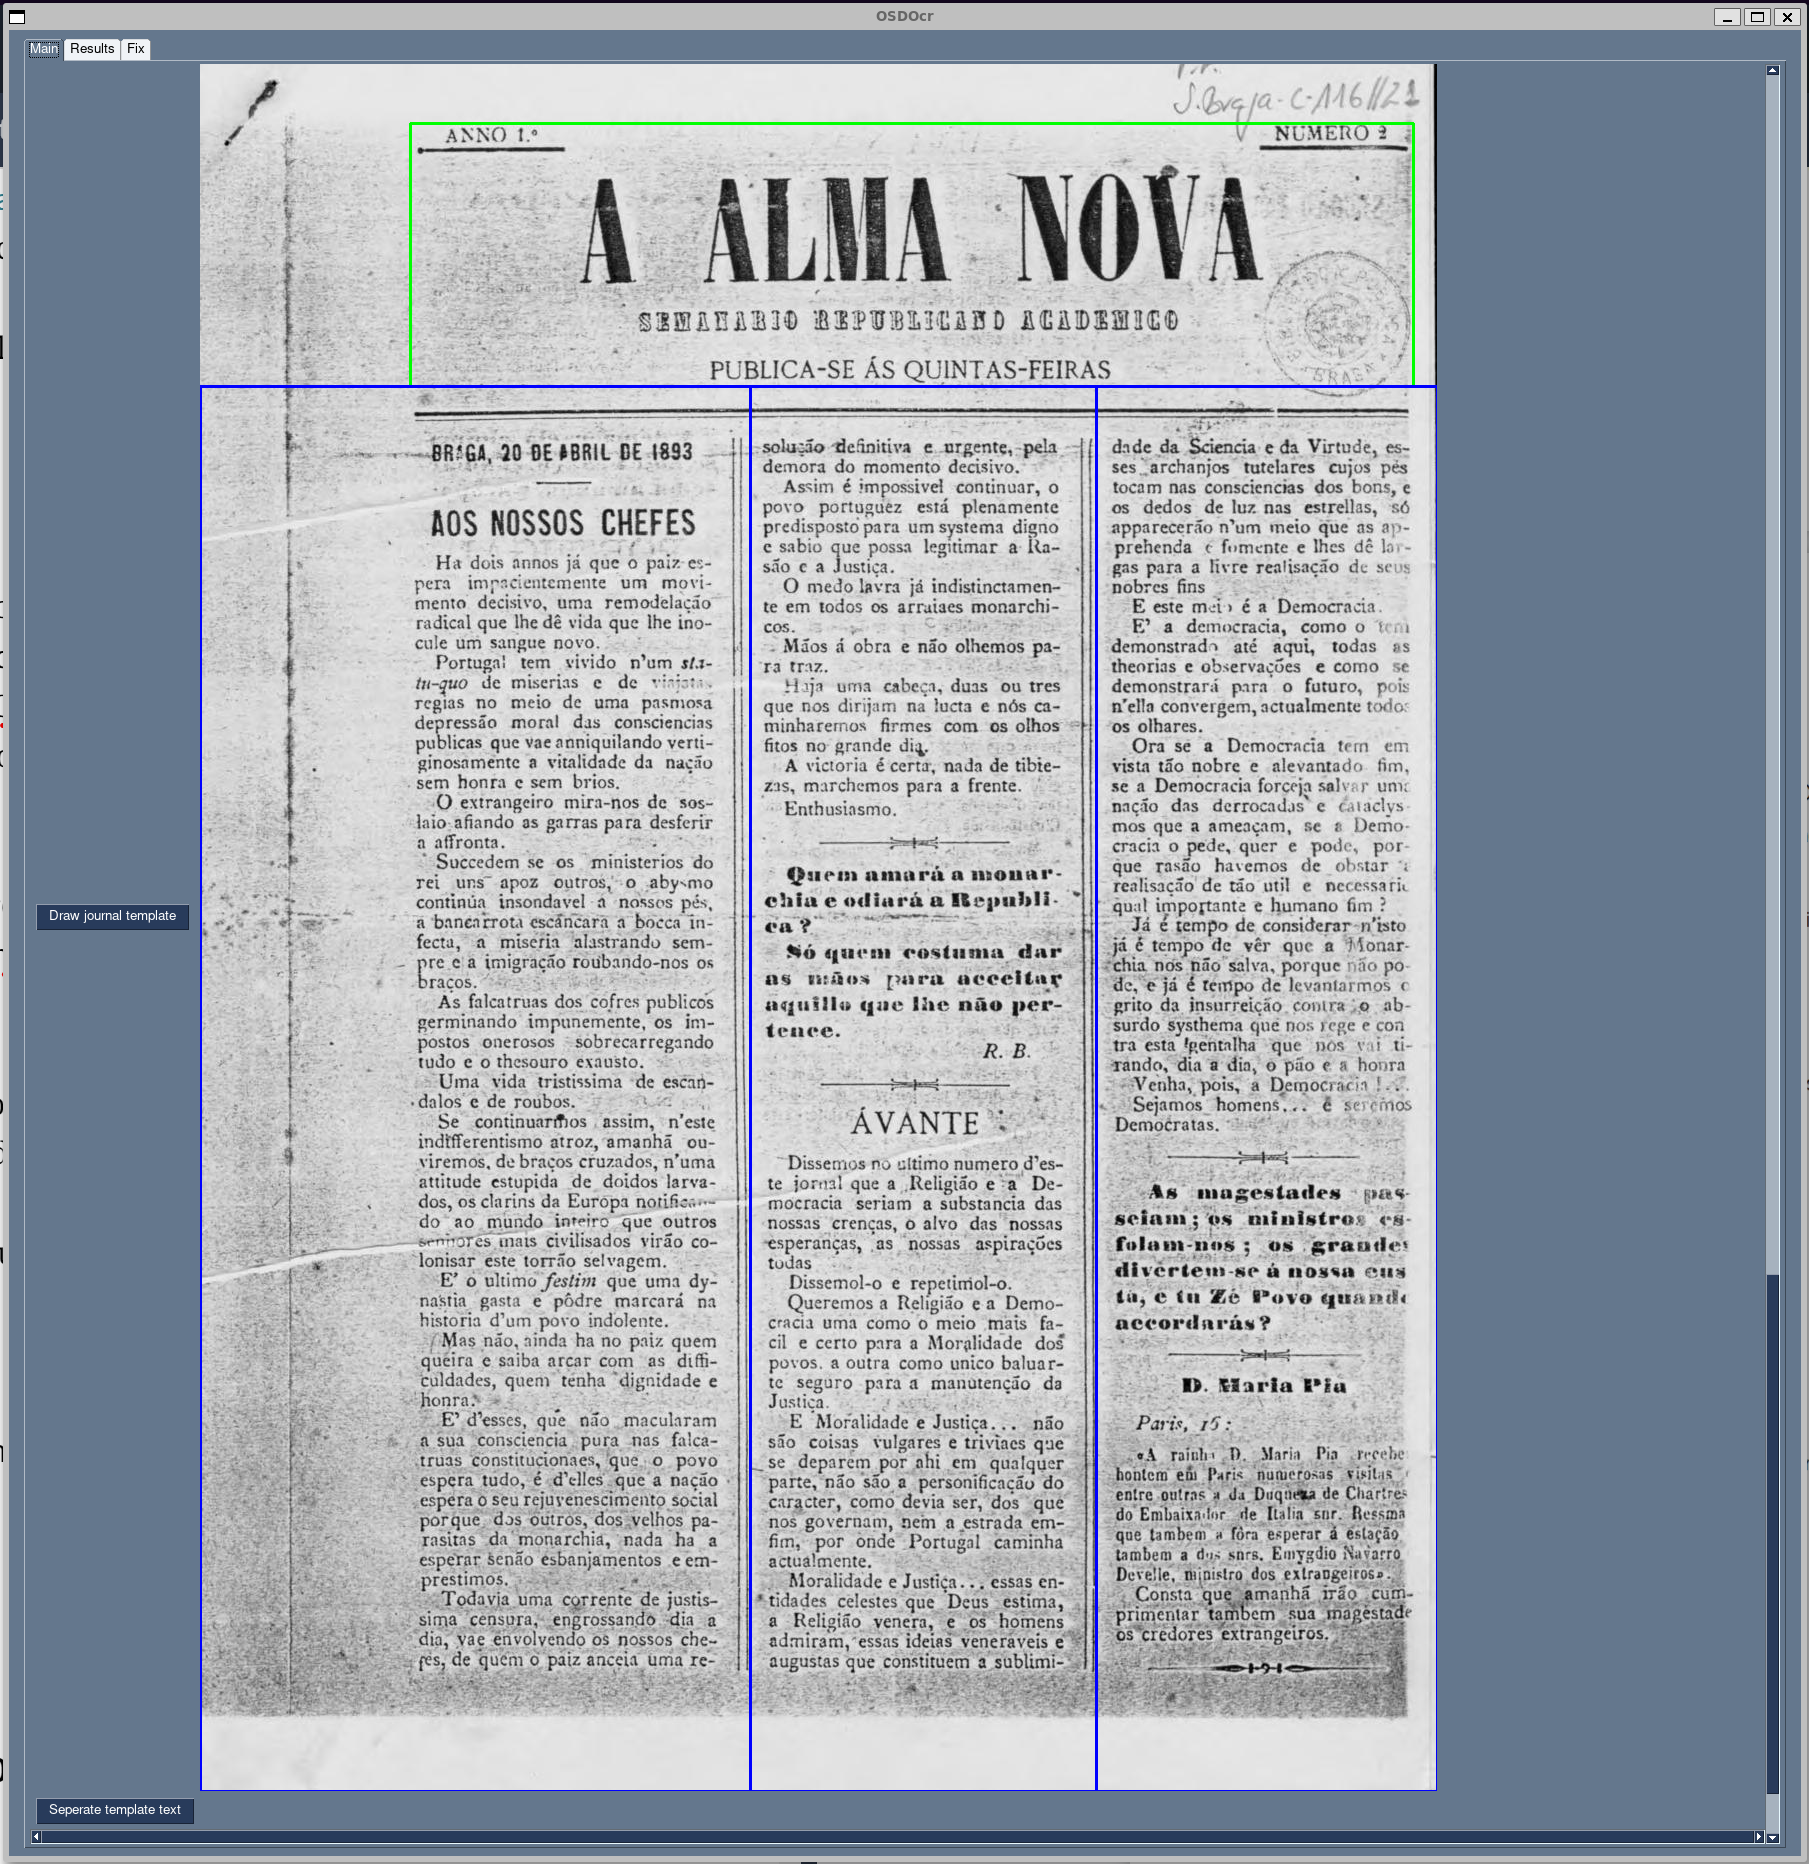
\includegraphics[width=1\textwidth]{images/implementacao/gui/gui_draw_template.png}
%     \caption{Visualização do cálculo do template de jornal}
%     \label{fig:gui_draw_template}
% \end{figure}
% 
% O cálculo de template é feito através da deteção e análise dos delimitadores dos resultados OCR. Áreas são depois calculadas de acordo com estes delimitadores e, como se pode ver no caso do Header (caixa a verde) da imagem \ref{fig:gui_draw_template}, a área é ajustada de acordo com as caixas com texto da respetiva área.
% 
% \subsubsection{Extração de artigos}
% 
% \begin{figure}[H]
%     \centering
%     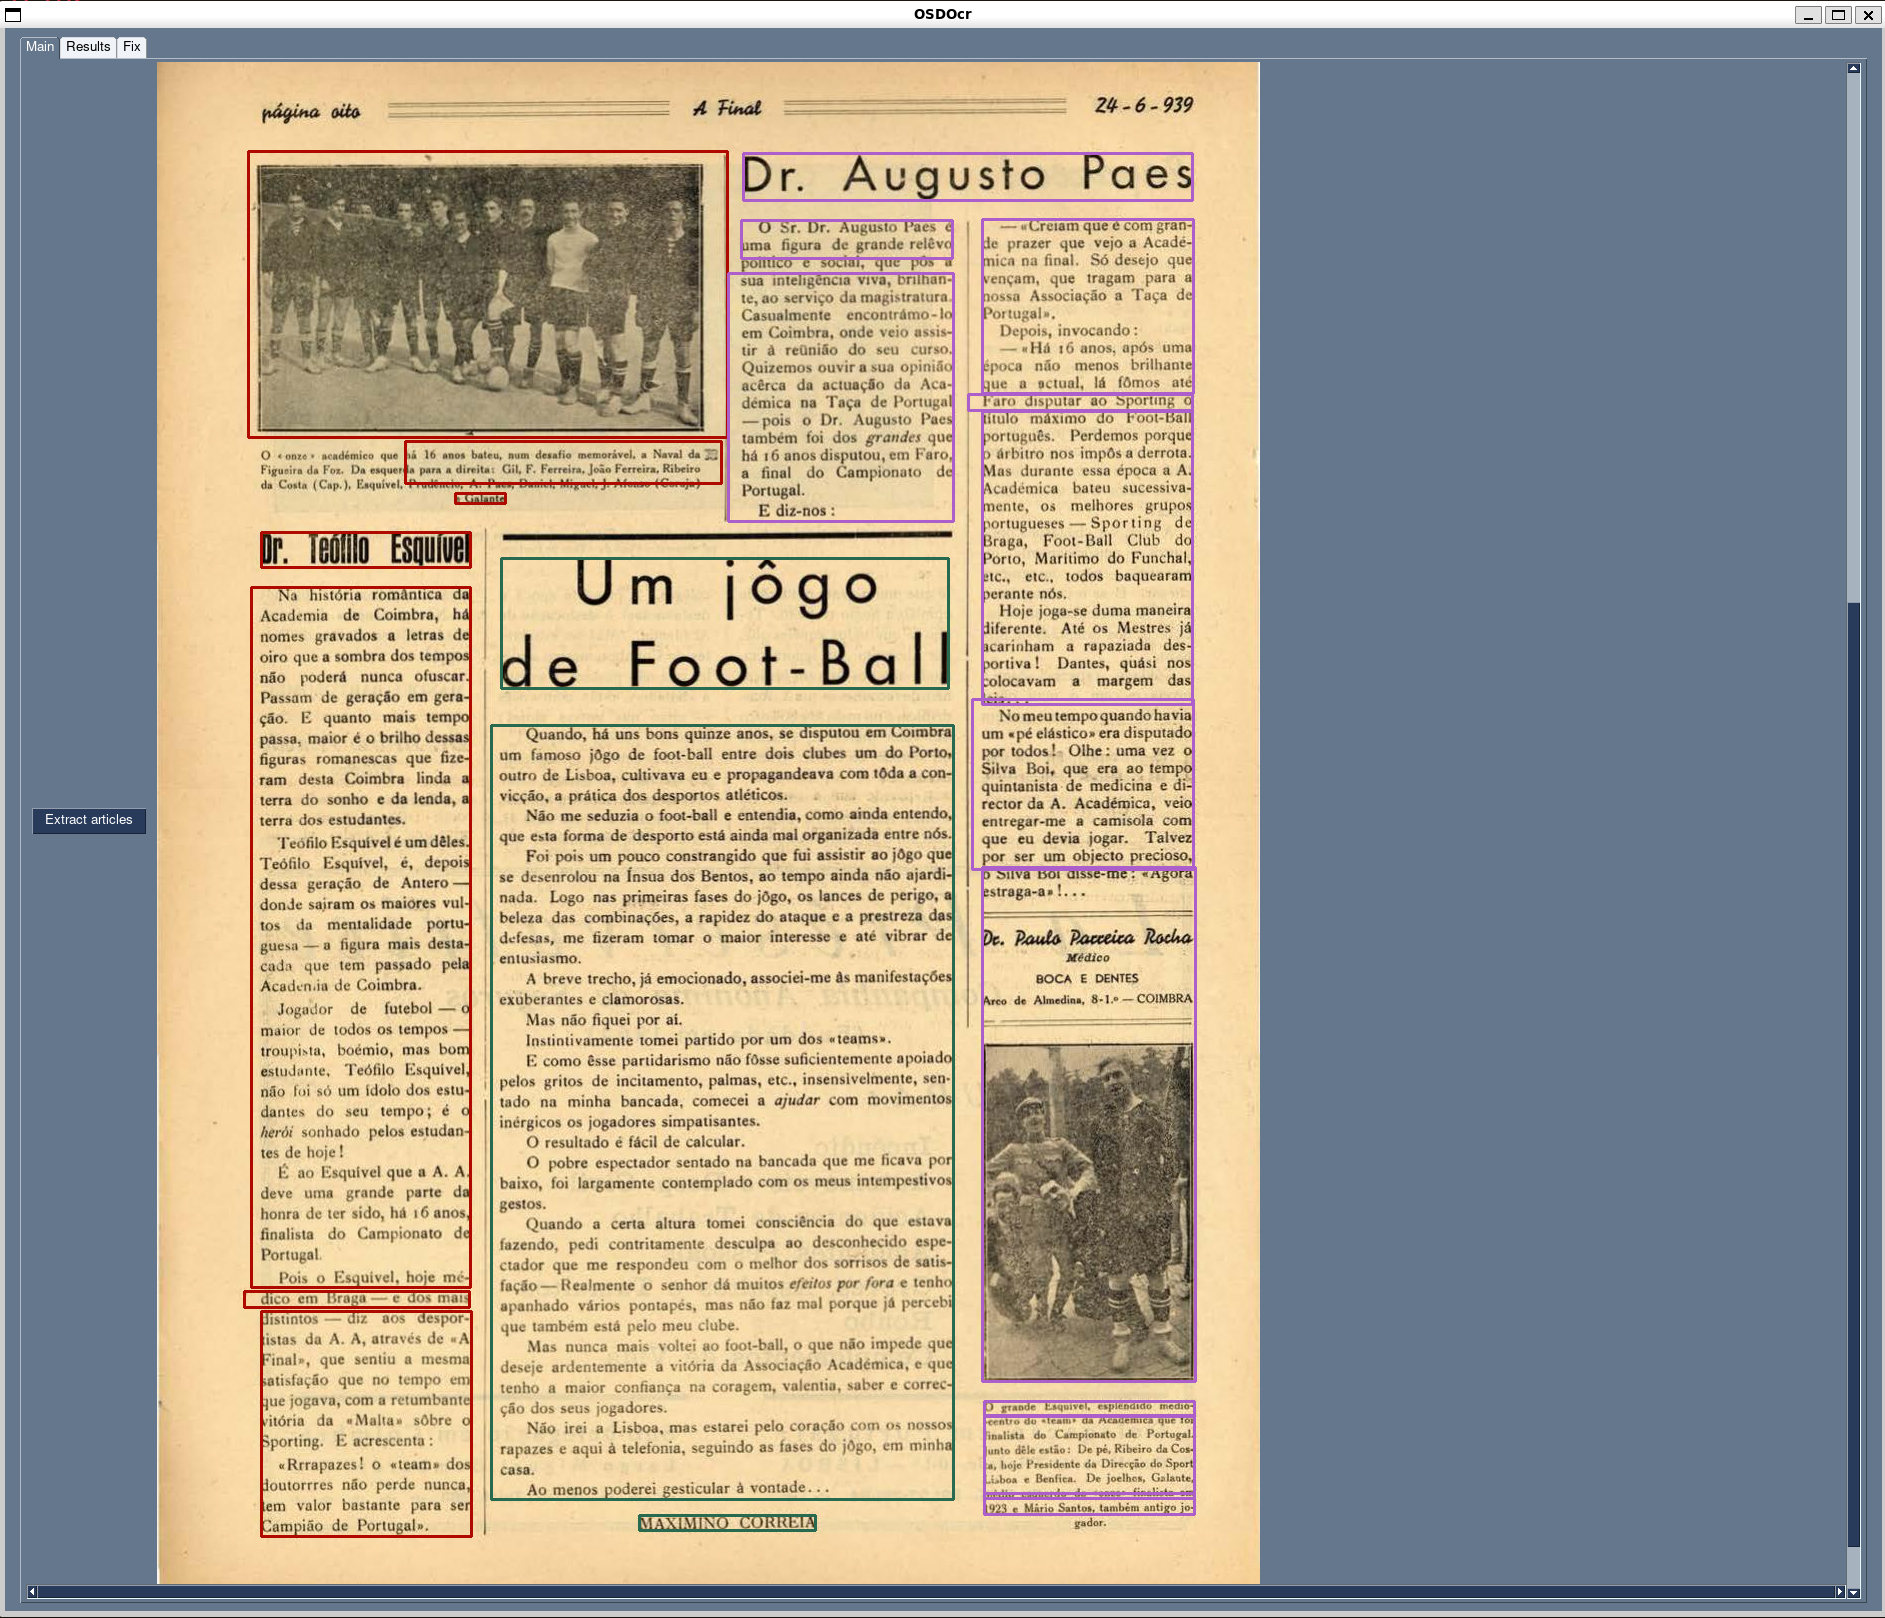
\includegraphics[width=1\textwidth]{images/implementacao/gui/gui_draw_articles.png}
%     \caption{Visualização dos artigos extraídos}
%     \label{fig:gui_draw_article}
% \end{figure}
% 
% Neste caso, os artigos são calculados e posteriormente escolhidas cores distintas para realçar cada um destes. Os artigos são representados pelo conjunto de blocos que foram agrupados como sendo um dado artigo.
% 
% \subsubsection{Limpeza de bounding boxes}
% 
% \begin{figure}[H]
%     \centering
%     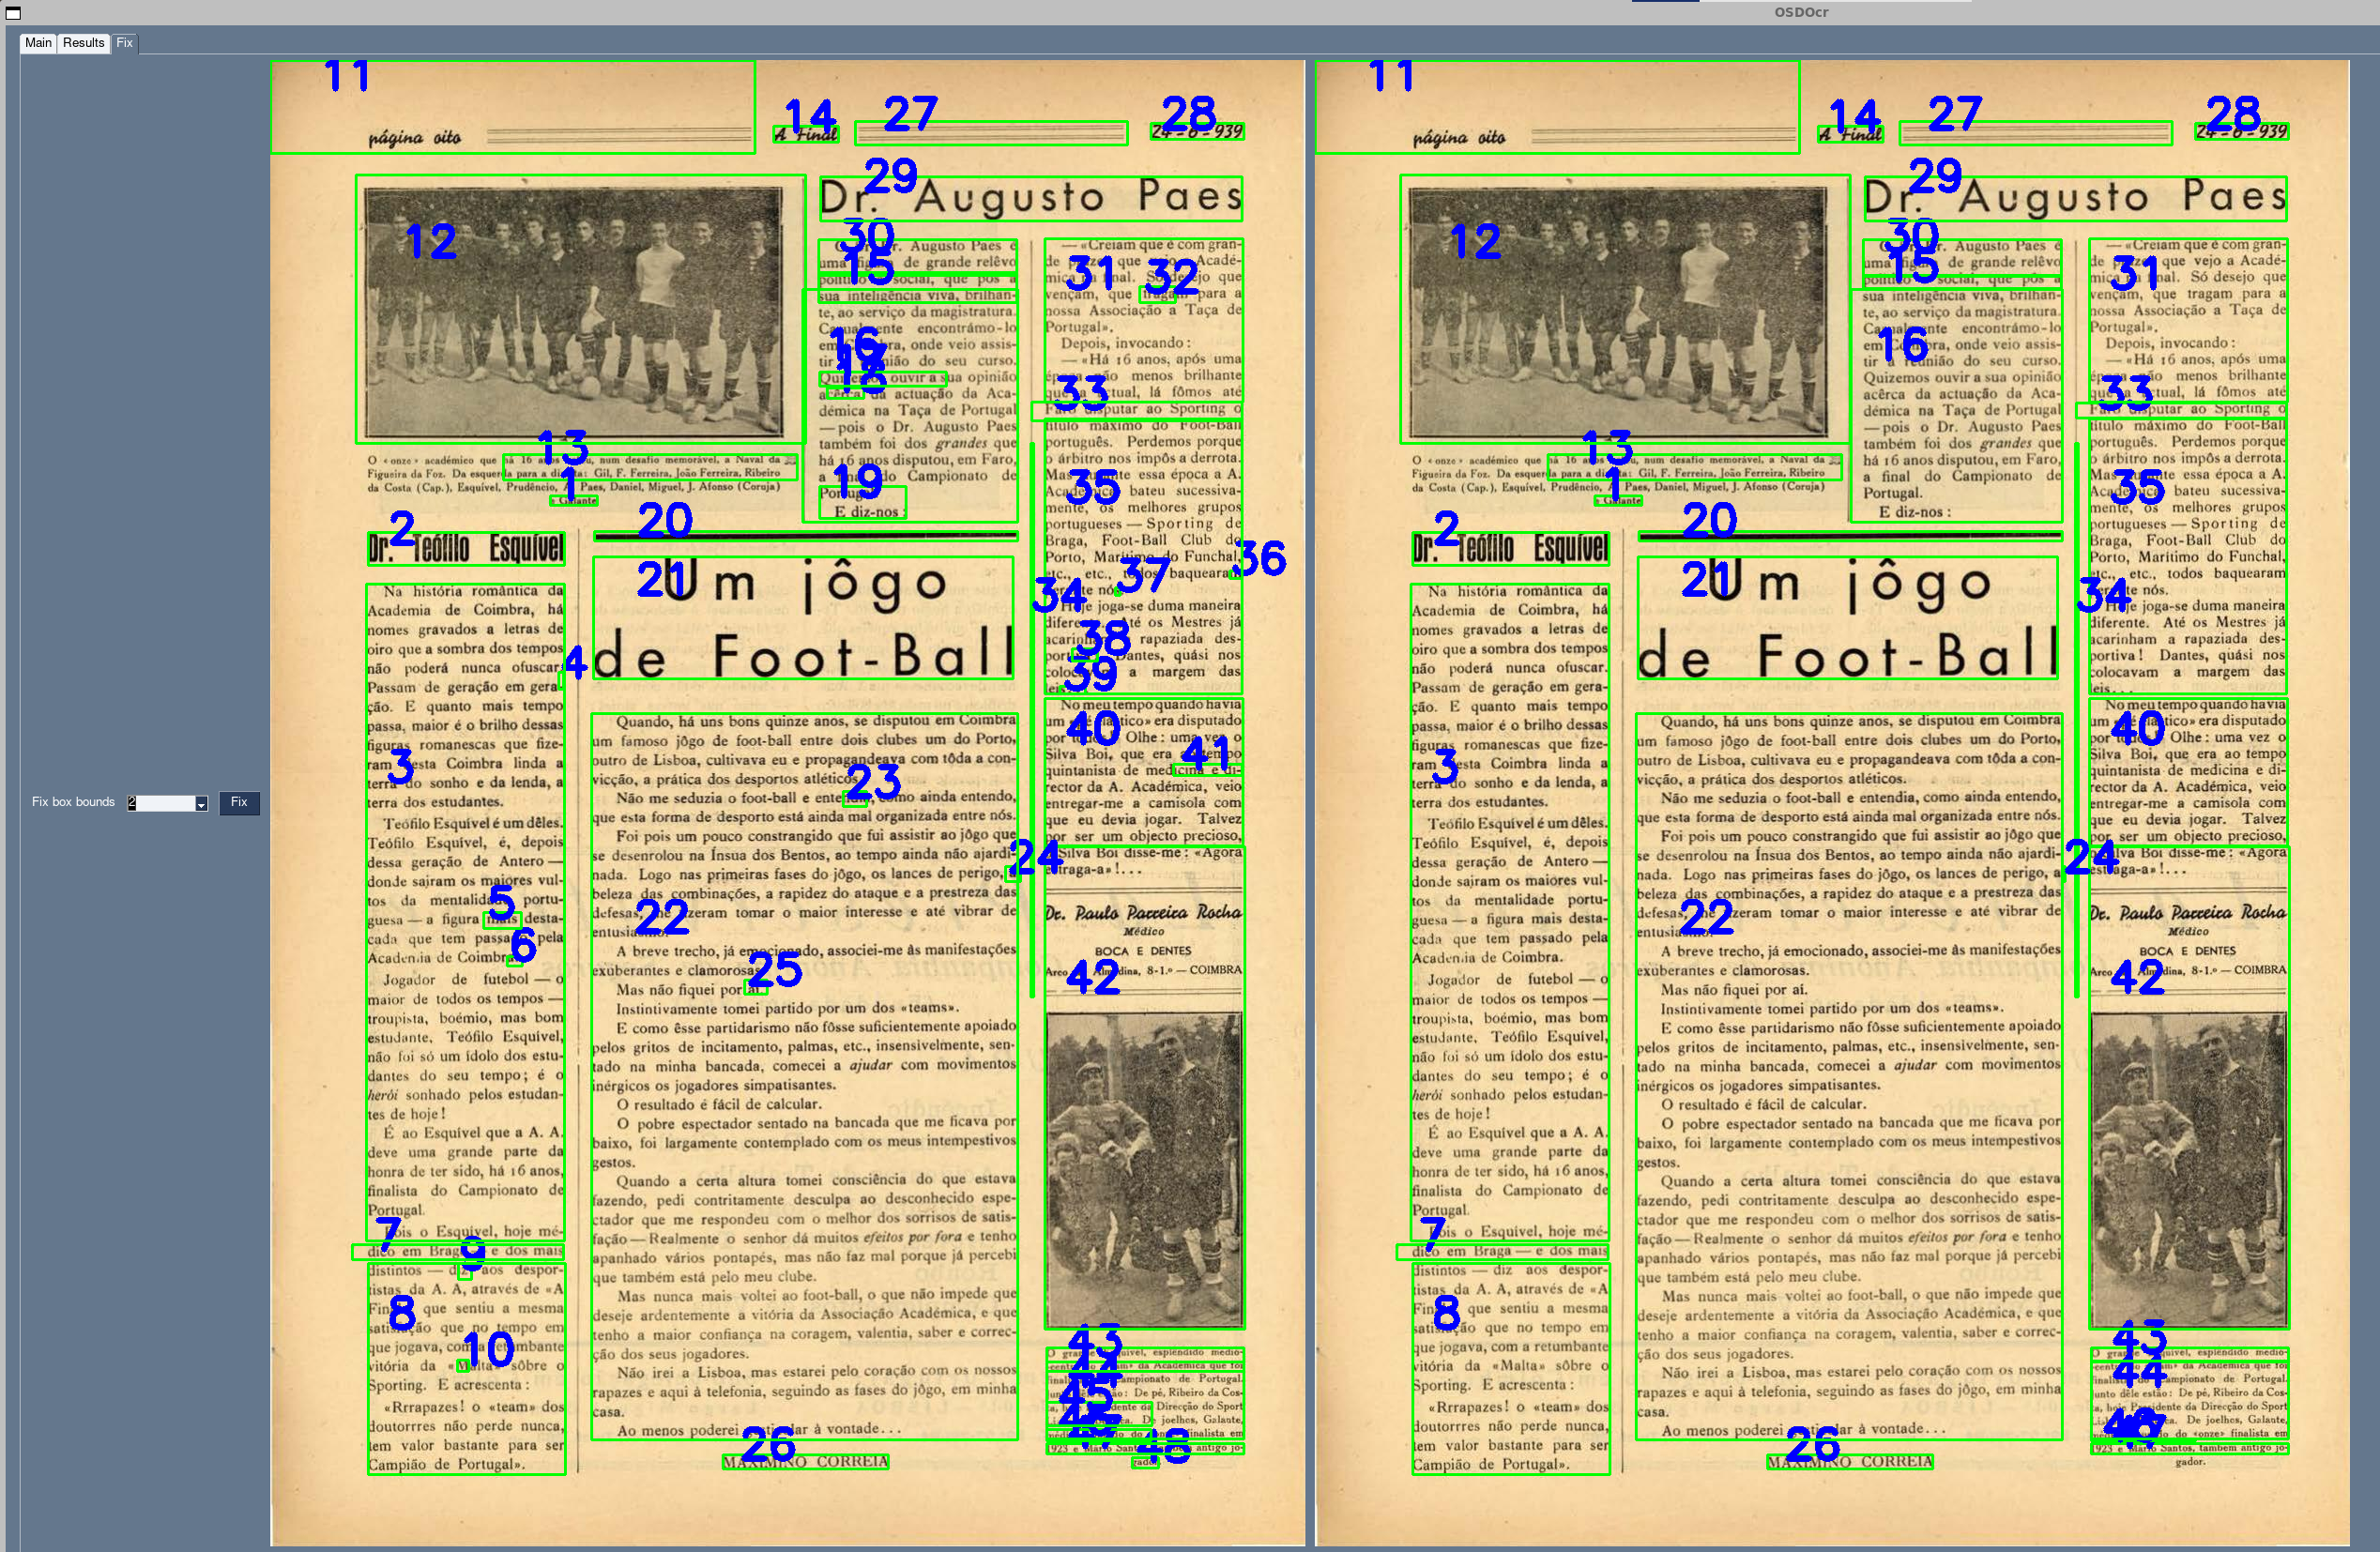
\includegraphics[width=1\textwidth]{images/implementacao/gui/gui_fix_blocks.png}
%     \caption{Visualização da limpeza de blocos}
%     \label{fig:gui_fix_bb}
% \end{figure}
% 
% Para facilitar a deteção das diferenças entre o antes e depois da limpeza, os dois estados são postos lado a lado e os blocos são identificados, mantendo a mesma identificação após a limpeza. 




